% Source: graduate-coursework/Research/Intro_to_Agents/handouts/Part7_Parallelization.tex

\documentclass[border=4pt]{standalone}
\usepackage{amsmath,amssymb,amsfonts}
\usepackage[T1]{fontenc}
\usepackage{graphicx}
\usepackage{lmodern}
\usepackage{tikz}
\usepackage{xcolor}
\usetikzlibrary{shapes.geometric, arrows.meta, positioning, calc, fit, backgrounds, matrix, decorations.pathreplacing}

\definecolor{UofSCGarnet}{HTML}{73000a}
\definecolor{UofSCBlack}{HTML}{000000}
\definecolor{UofSCWhite}{HTML}{ffffff}
\definecolor{UofSCRose}{HTML}{CC2E40}
\definecolor{UofSCAtlantic}{HTML}{466A9F}
\definecolor{UofSCCongaree}{HTML}{1F414D}
\definecolor{UofSCHorseshoe}{HTML}{65780B}
\definecolor{UofSCGrass}{HTML}{CED318}
\definecolor{UofSCHoneycomb}{HTML}{A49137}
\definecolor{UofSC90Black}{HTML}{363636}
\definecolor{UofSC70Black}{HTML}{5C5C5C}
\definecolor{UofSC50Black}{HTML}{A2A2A2}
\definecolor{UofSCWarmGrey}{HTML}{676156}
\definecolor{UofSCSandstorm}{HTML}{FFF2E3}
\definecolor{UofSCDarkGarnet}{HTML}{570008}
\definecolor{UofSCAzalea}{HTML}{844247}

\tikzset{
    % Node styles - all with sharp corners
    agentbox/.style={
        rectangle,
        draw=UofSCGarnet,
        fill=UofSCSandstorm,
        thick,
        minimum width=2cm,
        minimum height=0.8cm,
        text centered,
        font=\footnotesize
    },
    processbox/.style={
        rectangle,
        draw=UofSCAtlantic,
        fill=UofSCWhite,
        thick,
        minimum width=2.5cm,
        minimum height=0.7cm,
        text centered,
        font=\footnotesize
    },
    syncbox/.style={
        rectangle,
        draw=UofSCCongaree,
        fill=UofSCCongaree!20,
        thick,
        minimum width=3cm,
        minimum height=0.5cm,
        text centered,
        font=\footnotesize\bfseries
    },
    resultbox/.style={
        rectangle,
        draw=UofSCHorseshoe,
        fill=UofSCGrass!30,
        thick,
        minimum width=2cm,
        minimum height=0.7cm,
        text centered,
        font=\footnotesize
    },
    % Arrow styles
    myarrow/.style={
        ->,
        >=Stealth,
        thick,
        UofSCBlack
    },
    dashedarrow/.style={
        ->,
        >=Stealth,
        thick,
        dashed,
        UofSC70Black
    },
    % Timeline styles
    timeline/.style={
        draw=UofSCBlack,
        thick,
        ->,
        >=Stealth
    },
    timeblock/.style={
        rectangle,
        draw=none,
        minimum height=0.5cm,
        text centered,
        font=\tiny
    }
}

\begin{document}
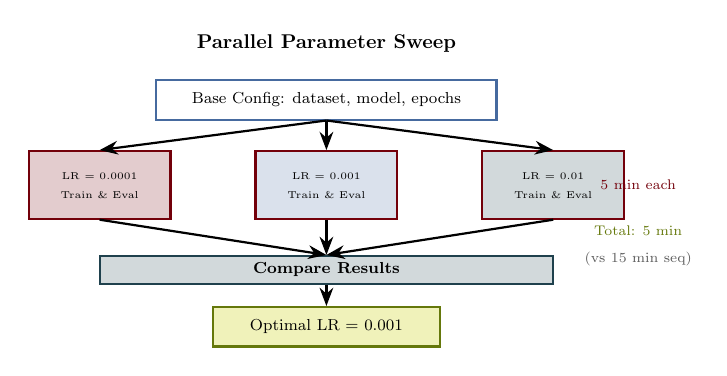
\begin{tikzpicture}[scale=0.72, transform shape]
            % Parameter sweep visualization
            \node[font=\bfseries] at (5.5,4) {Parallel Parameter Sweep};

            % Base config
            \node[processbox,minimum width=6cm] (base) at (5.5,3) {Base Config: dataset, model, epochs};

            % Three experiments
            \node[agentbox,fill=UofSCGarnet!20,minimum width=2.5cm,minimum height=1.2cm] (e1) at (1.5,1.5) {
                \begin{tabular}{c}
                    \tiny LR = 0.0001 \\
                    \tiny Train \& Eval
                \end{tabular}
            };
            \node[agentbox,fill=UofSCAtlantic!20,minimum width=2.5cm,minimum height=1.2cm] (e2) at (5.5,1.5) {
                \begin{tabular}{c}
                    \tiny LR = 0.001 \\
                    \tiny Train \& Eval
                \end{tabular}
            };
            \node[agentbox,fill=UofSCCongaree!20,minimum width=2.5cm,minimum height=1.2cm] (e3) at (9.5,1.5) {
                \begin{tabular}{c}
                    \tiny LR = 0.01 \\
                    \tiny Train \& Eval
                \end{tabular}
            };

            % Sync
            \node[syncbox,minimum width=8cm] (sync) at (5.5,0) {Compare Results};

            % Result
            \node[resultbox,minimum width=4cm] (result) at (5.5,-1) {Optimal LR = 0.001};

            % Arrows
            \draw[myarrow] (base.south) -- (e1.north);
            \draw[myarrow] (base.south) -- (e2.north);
            \draw[myarrow] (base.south) -- (e3.north);
            \draw[myarrow] (e1.south) -- (sync.north);
            \draw[myarrow] (e2.south) -- (sync.north);
            \draw[myarrow] (e3.south) -- (sync.north);
            \draw[myarrow] (sync.south) -- (result.north);

            % Timing
            \node[font=\scriptsize,UofSCGarnet] at (11,1.5) {5 min each};
            \node[font=\scriptsize,UofSCHorseshoe] at (11,0.7) {Total: 5 min};
            \node[font=\scriptsize,UofSC70Black] at (11,0.2) {(vs 15 min seq)};
        \end{tikzpicture}
\end{document}
